\documentclass[11pt]{article}

\usepackage[margin=0.82in]{geometry}
\usepackage[T1]{fontenc}
\usepackage[utf8]{inputenc}
\usepackage{lmodern}
\usepackage{microtype}
\usepackage{amsmath,amssymb,mathtools}
\usepackage{booktabs,longtable,array,tabularx}
\usepackage[table]{xcolor}
\usepackage{enumitem}
\usepackage{hyperref}
\usepackage{tikz}
\usepackage{pgfplots}
\usepackage[most]{tcolorbox}
\usepackage{caption}
\usepackage{float}
\usepackage{fancyhdr}
\usepackage{titlesec}

\usetikzlibrary{arrows.meta,positioning,fit,calc,shapes.geometric,decorations.pathreplacing}
\pgfplotsset{compat=1.18}

\definecolor{navy}{RGB}{19,35,59}
\definecolor{ink}{RGB}{33,48,71}
\definecolor{slate}{RGB}{82,98,122}
\definecolor{teal}{RGB}{24,169,153}
\definecolor{tealdark}{RGB}{12,127,117}
\definecolor{tealpale}{RGB}{221,244,241}
\definecolor{blue}{RGB}{59,130,246}
\definecolor{bluepale}{RGB}{231,240,254}
\definecolor{purple}{RGB}{139,92,246}
\definecolor{purplepale}{RGB}{238,232,255}
\definecolor{coral}{RGB}{242,107,91}
\definecolor{coralpale}{RGB}{253,233,230}
\definecolor{gold}{RGB}{244,185,66}
\definecolor{goldpale}{RGB}{255,243,214}
\definecolor{green}{RGB}{67,170,106}
\definecolor{greenpale}{RGB}{229,245,233}
\definecolor{pale}{RGB}{244,247,250}
\definecolor{mid}{RGB}{215,224,232}

\hypersetup{
  colorlinks=true,
  linkcolor=tealdark,
  urlcolor=blue!65!black,
  citecolor=purple!70!black,
  pdftitle={Bayesian Models from Scratch: A High-School Companion to ShapeMix-ATAC},
  pdfauthor={Andy Zhuang},
  pdfsubject={Bayesian foundations for understanding the ShapeMix-ATAC model},
  pdfkeywords={Bayesian model, prior, likelihood, posterior, MAP, negative binomial, multinomial, ShapeMix, ATAC-seq}
}

\setlength{\headheight}{14pt}
\setlength{\parindent}{0pt}
\setlength{\parskip}{0.45em}
\renewcommand{\arraystretch}{1.18}
\pagestyle{fancy}
\fancyhf{}
\lhead{Bayesian basics for ShapeMix-ATAC}
\rhead{High-school companion}
\cfoot{\thepage}

\titleformat{\section}{\Large\bfseries\color{navy}}{\thesection}{0.65em}{}
\titleformat{\subsection}{\large\bfseries\color{tealdark}}{\thesubsection}{0.65em}{}
\titleformat{\subsubsection}{\normalsize\bfseries\color{purple}}{\thesubsubsection}{0.65em}{}

\newcolumntype{L}[1]{>{\raggedright\arraybackslash}p{#1}}
\newcolumntype{C}[1]{>{\centering\arraybackslash}p{#1}}

\newcommand{\NB}{\operatorname{NegBinomial}}
\newcommand{\Mult}{\operatorname{Multinomial}}
\newcommand{\Gam}{\operatorname{Gamma}}
\newcommand{\Pois}{\operatorname{Poisson}}
\newcommand{\E}{\mathbb{E}}
\newcommand{\Var}{\operatorname{Var}}
\newcommand{\given}{\,|\,}
\newcommand{\term}[1]{\textbf{\color{tealdark}#1}}

\newtcolorbox{bigidea}{
  colback=bluepale,
  colframe=blue!75!black,
  title=Big idea,
  fonttitle=\bfseries,
  breakable
}
\newtcolorbox{checkpoint}{
  colback=greenpale,
  colframe=green!70!black,
  title=Check your understanding,
  fonttitle=\bfseries,
  breakable
}
\newtcolorbox{watchout}{
  colback=coralpale,
  colframe=coral!80!black,
  title=Watch out,
  fonttitle=\bfseries,
  breakable
}
\newtcolorbox{worked}[1]{
  colback=goldpale,
  colframe=gold!85!black,
  title=#1,
  fonttitle=\bfseries,
  breakable
}
\newtcolorbox{mathbox}[1]{
  colback=white,
  colframe=purple,
  title=#1,
  fonttitle=\bfseries,
  breakable
}
\newtcolorbox{translation}{
  colback=tealpale,
  colframe=tealdark,
  title=Translate the mathematics,
  fonttitle=\bfseries,
  breakable
}

\begin{document}
\hypersetup{pageanchor=false}

\begin{titlepage}
\centering
\vspace*{0.35in}
{\Huge\bfseries\color{navy} Bayesian Models from Scratch\par}
\vspace{0.18in}
{\LARGE\color{tealdark} A high-school companion to ShapeMix-ATAC\par}
\vspace{0.25in}
{\large No calculus required: pictures, small-number examples, and equation-reading practice\par}

\vspace{0.55in}
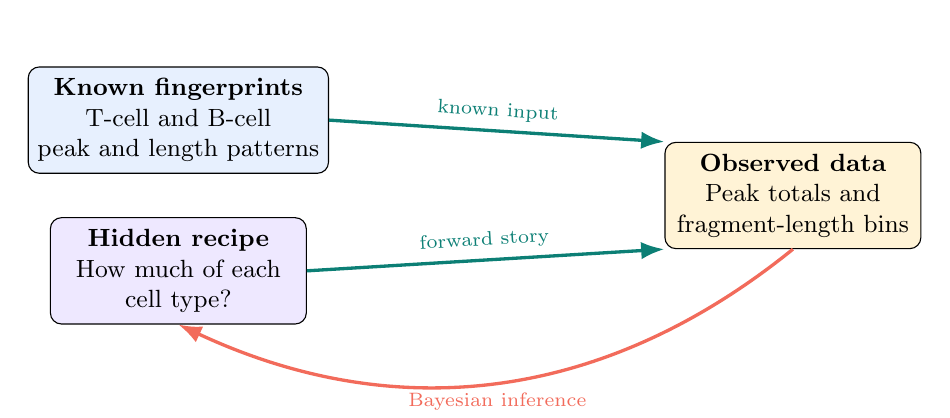
\begin{tikzpicture}[>=Latex,every node/.style={align=center,font=\small}]
  \node[draw,rounded corners,fill=bluepale,minimum width=3.25cm,minimum height=1.35cm] (ref) {
    \textbf{Known fingerprints}\\
    T-cell and B-cell\\
    peak and length patterns
  };
  \node[draw,rounded corners,fill=purplepale,minimum width=3.25cm,minimum height=1.35cm,below=0.55cm of ref] (mix) {
    \textbf{Hidden recipe}\\
    How much of each\\
    cell type?
  };
  \coordinate (leftmid) at ($(ref.east)!0.5!(mix.east)$);
  \node[draw,rounded corners,fill=goldpale,minimum width=3.25cm,minimum height=1.35cm,right=4.4cm of leftmid] (data) {
    \textbf{Observed data}\\
    Peak totals and\\
    fragment-length bins
  };
  \draw[->,very thick,tealdark] (ref.east) -- node[above,sloped,font=\scriptsize]{known input} (data.north west);
  \draw[->,very thick,tealdark] (mix.east) -- node[above,sloped,font=\scriptsize]{forward story} (data.south west);
  \draw[->,very thick,coral,bend left=32] (data.south) to node[below,font=\scriptsize]{Bayesian inference} (mix.south);
\end{tikzpicture}

\vfill
\begin{bigidea}
This tutorial prepares you to read
\texttt{ShapeMix\_ATAC\_Bayesian\_Model\_Tutorial.pdf}.
You will learn what a model is, how Bayes' rule updates a belief, why counts need
probability distributions, how mixtures are represented, and what a MAP estimate
does. Every new symbol is translated into ordinary language.
\end{bigidea}

\vfill
{\large Companion tutorial, version 1.0\par}
{\large August 2026\par}
\end{titlepage}

\hypersetup{pageanchor=true}
\pagenumbering{roman}
\setcounter{tocdepth}{1}
\tableofcontents
\newpage
\pagenumbering{arabic}

\section{How to use this tutorial}

This document is a \emph{prequel}, not a replacement for the full ShapeMix
tutorial. Read it in order the first time. Keep a pencil nearby and actually try
the short checkpoints before reading their answers.

\begin{center}
\begin{tabularx}{0.94\linewidth}{L{0.23\linewidth}X}
\toprule
If you want to learn \ldots & Focus on \ldots \\
\midrule
Bayes' rule itself & Sections 3--4 \\
Why special distributions are used & Section 5 \\
How mixtures are inferred & Sections 6 and 9 \\
The ShapeMix symbols and equations & Sections 8--10 \\
What MAP means & Section 12 \\
How to approach the original PDF & Section 14 \\
\bottomrule
\end{tabularx}
\end{center}

\subsection{What you need before starting}

You should be comfortable with fractions, percentages, multiplication, and simple
algebra. Summation notation such as \(\sum\) will be explained. You do not need
calculus, programming, or previous statistics.

\begin{checkpoint}
By the end, you should be able to explain this sentence:

\begin{quote}
ShapeMix combines a negative-binomial model for the number of cut sites in a peak,
a conditional multinomial model for how those cuts split among parent-fragment
length bins, and a Gamma prior on positive cell-type abundances; it reports the
MAP mixture.
\end{quote}
\end{checkpoint}

\section{Start with the scientific question}

\subsection{What is observed, and what is hidden?}

In spatial ATAC-seq, a tissue location can contain material from several cell
types. The experiment gives us counts at that location, but it does not label each
count with the cell type that produced it.

\begin{center}
\begin{tabularx}{0.92\linewidth}{L{0.25\linewidth}X}
\toprule
Role & ShapeMix example \\
\midrule
\term{Observed data} & Cut-site counts in genomic peaks, grouped by the length of each cut site's parent fragment. \\
\term{Known inputs} & Reference fingerprints learned from labeled training cells. \\
\term{Hidden quantity} & The amount of each cell type in the mixed spot. \\
\term{Reported answer} & The estimated cell-type proportions. \\
\bottomrule
\end{tabularx}
\end{center}

\begin{figure}[H]
\centering
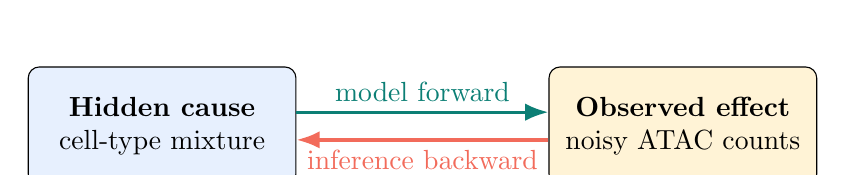
\begin{tikzpicture}[>=Latex,every node/.style={align=center}]
  \node[draw,rounded corners,fill=bluepale,minimum width=3.4cm,minimum height=1.5cm] (hidden) {
    \textbf{Hidden cause}\\
    cell-type mixture
  };
  \node[draw,rounded corners,fill=goldpale,minimum width=3.4cm,minimum height=1.5cm,right=3.2cm of hidden] (seen) {
    \textbf{Observed effect}\\
    noisy ATAC counts
  };
  \draw[->,very thick,tealdark] ([yshift=5pt]hidden.east) -- node[above]{model forward} ([yshift=5pt]seen.west);
  \draw[->,very thick,coral] ([yshift=-5pt]seen.west) -- node[below]{inference backward} ([yshift=-5pt]hidden.east);
\end{tikzpicture}
\caption{A model describes how a hidden cause could produce an observed effect. Inference asks which hidden causes are supported by the effect we actually observed.}
\end{figure}

\subsection{A model is a precise story}

A \term{model} is not the data and it is not the answer. It is a set of rules that
connect possible hidden explanations to possible observations.

For ShapeMix, the story is approximately:

\begin{enumerate}[leftmargin=2em]
  \item A spot has some effective amount of each cell type.
  \item Each cell type has a known reference fingerprint across peaks and length bins.
  \item Mixing those fingerprints gives expected peak totals and expected length proportions.
  \item Random experimental variation makes the observed counts differ from those expectations.
\end{enumerate}

\begin{bigidea}
A Bayesian model first tells a story in the easy direction:
\[
\text{hidden mixture}\longrightarrow\text{expected signal}\longrightarrow\text{noisy data}.
\]
Bayesian inference uses the observed data to reason in the reverse direction.
\end{bigidea}

\subsection{One ATAC counting detail}

A deduplicated ATAC fragment has two ends, corresponding to two Tn5 cut-site
observations. Each end is assigned independently to a peak. Therefore one fragment
can contribute two cuts to one peak, one cut to each of two peaks, one selected
cut, or no selected cuts.

For a simple classroom picture, we can assume both ends of every drawn fragment
land in the same peak. Under that assumption:
\[
12\text{ fragments}\times2\text{ ends per fragment}=24\text{ cut-site counts}.
\]

\begin{watchout}
ShapeMix's primary count unit is a \emph{cut site tagged by the length of its parent
fragment}, not a unique fragment. Keeping that distinction straight prevents a
factor-of-two counting mistake.
\end{watchout}

\section{Probability is a language for uncertainty}

\subsection{Probabilities are numbers from 0 to 1}

A probability of \(0\) means impossible, \(1\) means certain, and \(0.60\) means
60\%. Imagine 100 equally likely cards: 60 teal cards and 40 gray cards.

\begin{figure}[H]
\centering
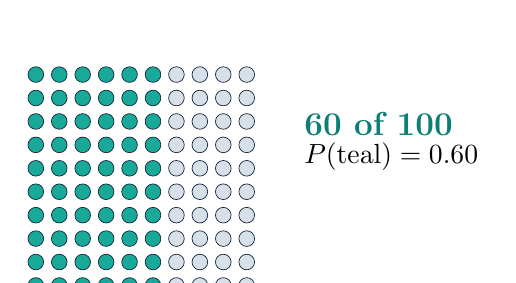
\begin{tikzpicture}[scale=0.62]
  \foreach \x in {0,...,5}{
    \foreach \y in {0,...,9}{
      \filldraw[fill=teal,draw=navy,line width=0.25pt] (\x*0.48,\y*0.48) circle (0.16);
    }
  }
  \foreach \x in {6,...,9}{
    \foreach \y in {0,...,9}{
      \filldraw[fill=mid,draw=navy,line width=0.25pt] (\x*0.48,\y*0.48) circle (0.16);
    }
  }
  \node[anchor=west,font=\large\bfseries,text=tealdark] at (5.3,3.3) {60 of 100};
  \node[anchor=west,font=\normalsize] at (5.3,2.65) {\(P(\text{teal})=0.60\)};
\end{tikzpicture}
\caption{Probability can be pictured as a fraction of equally likely possibilities.}
\end{figure}

The notation \(P(A)\) means the probability of event \(A\). For example,
\[
P(\text{short parent fragment})=0.60.
\]

\subsection{Conditional probability changes the question}

The vertical bar in \(P(A\mid B)\) is read as “given.” It means:

\begin{quote}
What is the probability of \(A\), if we already know \(B\)?
\end{quote}

Suppose a reference tells us:

\begin{center}
\begin{tabular}{L{0.27\linewidth}C{0.22\linewidth}C{0.22\linewidth}}
\toprule
Parent-fragment category & T-cell cut & B-cell cut \\
\midrule
Short & \(80\%\) & \(20\%\) \\
Long & \(20\%\) & \(80\%\) \\
\bottomrule
\end{tabular}
\end{center}

Then
\[
P(\text{short}\mid T)=0.80,
\qquad
P(\text{short}\mid B)=0.20.
\]
These numbers answer: “If the cut came from this cell type, how likely is a short
parent fragment?”

\begin{watchout}
\[
P(\text{short}\mid T)\neq P(T\mid\text{short}).
\]
The first predicts data from a known cell type. The second infers a cell type from
observed data. Bayes' rule connects the two directions.
\end{watchout}

\subsection{A probability tree}

Assume a cut is equally likely to come from a T cell or a B cell before we inspect
its parent-fragment length:
\[
P(T)=0.50,\qquad P(B)=0.50.
\]

\begin{figure}[H]
\centering
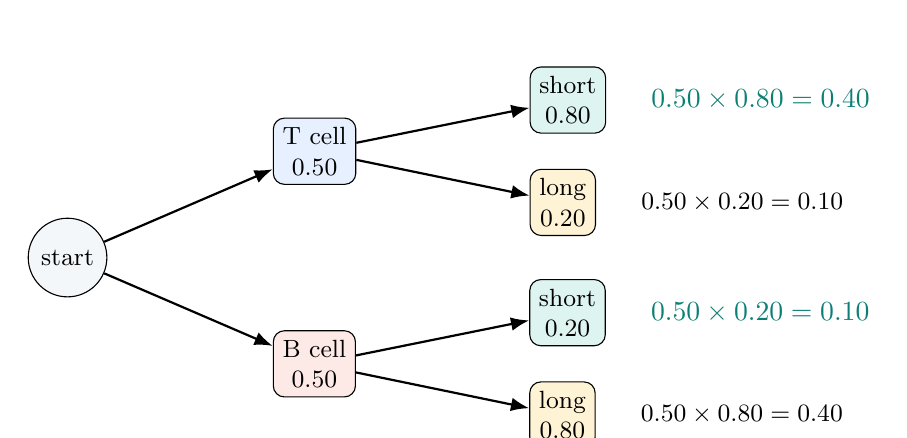
\begin{tikzpicture}[>=Latex,node distance=0.5cm,every node/.style={font=\small,align=center}]
  \node[draw,circle,fill=pale,minimum size=0.9cm] (start) {start};
  \node[draw,rounded corners,fill=bluepale,right=2.1cm of start,yshift=1.35cm] (t) {T cell\\\(0.50\)};
  \node[draw,rounded corners,fill=coralpale,right=2.1cm of start,yshift=-1.35cm] (b) {B cell\\\(0.50\)};
  \node[draw,rounded corners,fill=tealpale,right=2.2cm of t,yshift=0.65cm] (ts) {short\\\(0.80\)};
  \node[draw,rounded corners,fill=goldpale,right=2.2cm of t,yshift=-0.65cm] (tl) {long\\\(0.20\)};
  \node[draw,rounded corners,fill=tealpale,right=2.2cm of b,yshift=0.65cm] (bs) {short\\\(0.20\)};
  \node[draw,rounded corners,fill=goldpale,right=2.2cm of b,yshift=-0.65cm] (bl) {long\\\(0.80\)};
  \draw[->,thick] (start) -- (t);
  \draw[->,thick] (start) -- (b);
  \draw[->,thick] (t) -- (ts);
  \draw[->,thick] (t) -- (tl);
  \draw[->,thick] (b) -- (bs);
  \draw[->,thick] (b) -- (bl);
  \node[anchor=west,text=tealdark,font=\bfseries] at ($(ts.east)+(0.45,0)$) {\(0.50\times0.80=0.40\)};
  \node[anchor=west] at ($(tl.east)+(0.45,0)$) {\(0.50\times0.20=0.10\)};
  \node[anchor=west,text=tealdark,font=\bfseries] at ($(bs.east)+(0.45,0)$) {\(0.50\times0.20=0.10\)};
  \node[anchor=west] at ($(bl.east)+(0.45,0)$) {\(0.50\times0.80=0.40\)};
\end{tikzpicture}
\caption{Multiply along a branch. The two highlighted branches are the ways to observe a short-parent cut.}
\end{figure}

If we observe a short-parent cut, only the two short branches remain. Their weights
are \(0.40\) for T and \(0.10\) for B. Normalize them so they add to one:
\[
P(T\mid\text{short})=\frac{0.40}{0.40+0.10}=0.80.
\]

\begin{checkpoint}
Why is the answer 80\% rather than 40\%? Because 40\% is the probability of the
\emph{joint event} “T cell and short.” Once short has already been observed, we
renormalize within the short branches only.
\end{checkpoint}

\section{Bayes' rule: prior, likelihood, and posterior}

\subsection{The formula and its translation}

\begin{mathbox}{Bayes' rule}
\[
\boxed{
P(H\mid E)
=
\frac{P(E\mid H)P(H)}{P(E)}
}
\]
\[
\underbrace{P(H\mid E)}_{\text{posterior}}
=
\frac{
\underbrace{P(E\mid H)}_{\text{likelihood}}
\underbrace{P(H)}_{\text{prior}}
}{
\underbrace{P(E)}_{\text{evidence / normalizer}}
}.
\]
\end{mathbox}

Here \(H\) means a possible hidden explanation, or \term{hypothesis}, and \(E\)
means the observed \term{evidence}.

\begin{center}
\begin{tabularx}{0.95\linewidth}{L{0.18\linewidth}L{0.29\linewidth}X}
\toprule
Word & Question & Short-fragment example \\
\midrule
\term{Prior} & What was plausible before these data? & The next cut is equally likely to come from T or B. \\
\term{Likelihood} & If this explanation were true, how well would it predict the data? & T predicts short with 80\%; B predicts short with 20\%. \\
\term{Posterior} & What is plausible after seeing the data? & Given short, support becomes 80\% T and 20\% B. \\
\term{Evidence} & How common is the observation across all explanations? & \(0.40+0.10=0.50\); it normalizes the answer. \\
\bottomrule
\end{tabularx}
\end{center}

\begin{bigidea}
Bayes' rule is an update:
\[
\boxed{\text{posterior}\propto\text{likelihood}\times\text{prior}.}
\]
The symbol \(\propto\) means “proportional to.” It says the numerator gives
relative scores; dividing by the evidence makes the scores add to one.
\end{bigidea}

\subsection{A complete numerical update}

\begin{worked}{One observed short-parent cut}
Let \(H_T\) mean the cut came from a T cell and \(H_B\) mean it came from a B cell.

\[
\begin{array}{c|c|c|c}
\text{Hypothesis} & \text{prior} & \text{likelihood of short} & \text{unnormalized score}\\
\hline
H_T & 0.50 & 0.80 & 0.40\\
H_B & 0.50 & 0.20 & 0.10
\end{array}
\]

The scores total \(0.50\). Divide each score by \(0.50\):
\[
P(H_T\mid\text{short})=0.80,\qquad
P(H_B\mid\text{short})=0.20.
\]
\end{worked}

\subsection{What if the prior is not equal?}

Suppose that, before seeing this cut, we assign a 25\% prior probability to a
T-cell source:
\[
P(H_T)=0.25,\qquad P(H_B)=0.75.
\]
After one short-parent cut,
\[
P(H_T\mid\text{short})
=
\frac{0.80(0.25)}{0.80(0.25)+0.20(0.75)}
=
\frac{0.20}{0.35}
\approx0.57.
\]
The short cut moves support toward T, but the stronger B prior still matters.
This is a prior about the \emph{source of a cut}; it equals a source-cell fraction
only when the cell types have equal expected cut yields.

\begin{checkpoint}
Does a prior force the answer? No. A prior is one part of the score. Repeated
strong evidence can overwhelm a weak or moderate prior, while weak data leave
more room for the prior to matter.
\end{checkpoint}

\subsection{Probability versus likelihood}

The expression \(P(E\mid H)\) has two related readings:

\begin{itemize}[leftmargin=2em]
  \item If \(H\) is fixed and possible data \(E\) vary, it is a probability model for data.
  \item If the observed \(E\) is fixed and candidate explanations \(H\) vary, the same expression is called the \term{likelihood}; it scores the candidates.
\end{itemize}

\begin{watchout}
A likelihood is not automatically a probability distribution over hypotheses.
Multiplying by a prior and normalizing is what produces a posterior distribution
over hypotheses.
\end{watchout}

\subsection{Classification is not yet deconvolution}

The example above asked which \emph{single} cell type produced one cut.
ShapeMix asks a harder question: what \emph{mixture} of cell types produced many
cuts? The same logic survives, but the hypothesis becomes a continuous recipe
such as 67\% T and 33\% B.

\section{Probability distributions: rules for random outcomes}

\subsection{Random does not mean patternless}

A \term{random variable} is a number whose value can vary when an experiment is
repeated. A \term{probability distribution} lists or describes how plausible each
possible value is.

Suppose a model expects 10 cut sites at a peak. Repeating the experiment does not
force the count to be exactly 10 every time. We might observe 8, 11, 14, or another
nearby value. The distribution describes this variation.

\begin{center}
\begin{tabularx}{0.96\linewidth}{L{0.22\linewidth}L{0.28\linewidth}X}
\toprule
Distribution & What it describes & ShapeMix role \\
\midrule
\(\Pois\) & A basic nonnegative count whose variance equals its mean. & Useful comparison and software check. \\
\(\NB\) & A nonnegative count with extra variation beyond Poisson. & Models the total cut sites in a peak. \\
\(\Mult\) & How a fixed total is divided among categories. & Splits a peak total among short, middle, and long bins. \\
\(\Gam\) & A positive continuous quantity. & Prior for positive effective cell-type abundance. \\
\bottomrule
\end{tabularx}
\end{center}

\subsection{The symbol \texorpdfstring{\(\sim\)}{tilde}}

\[
X\sim\NB(\text{mean}=10,\text{inverse-dispersion}=2)
\]
is read:

\begin{quote}
The random count \(X\) follows a negative-binomial distribution with these settings.
\end{quote}

The symbol \(\sim\) does \emph{not} mean approximately equal here. It means
“is modeled as a random draw from.”

\subsection{Poisson versus negative binomial}

A Poisson distribution is a simple count model:
\[
\E[X]=\mu,\qquad \Var(X)=\mu.
\]
Real sequencing counts often vary more. The target ShapeMix model uses a negative
binomial parameterized by a mean \(\mu\) and an inverse-dispersion \(\phi\):
\[
\E[X]=\mu,\qquad
\Var(X)=\mu+\frac{\mu^2}{\phi}.
\]

\begin{figure}[H]
\centering
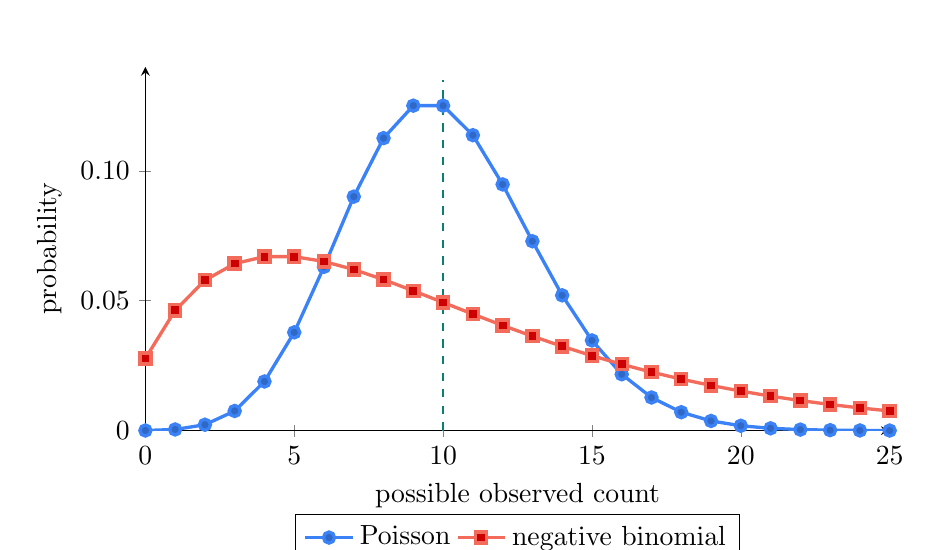
\begin{tikzpicture}
\begin{axis}[
  width=0.91\linewidth,
  height=6.2cm,
  xlabel={possible observed count},
  ylabel={probability},
  xmin=0,xmax=25,
  ymin=0,ymax=0.14,
  xtick={0,5,10,15,20,25},
  ytick={0,0.05,0.10},
  yticklabels={0,0.05,0.10},
  legend style={at={(0.5,-0.23)},anchor=north,legend columns=2},
  axis lines=left
]
\addplot+[very thick,blue,mark=*] coordinates {
  (0,0.00005) (1,0.00045) (2,0.00227) (3,0.00757) (4,0.01892)
  (5,0.03783) (6,0.06306) (7,0.09008) (8,0.11260) (9,0.12511)
  (10,0.12511) (11,0.11374) (12,0.09478) (13,0.07291) (14,0.05208)
  (15,0.03472) (16,0.02170) (17,0.01276) (18,0.00709) (19,0.00373)
  (20,0.00187) (21,0.00089) (22,0.00040) (23,0.00018) (24,0.00007) (25,0.00003)
};
\addplot+[very thick,coral,mark=square*] coordinates {
  (0,0.02778) (1,0.04630) (2,0.05787) (3,0.06430) (4,0.06698)
  (5,0.06698) (6,0.06512) (7,0.06202) (8,0.05814) (9,0.05384)
  (10,0.04935) (11,0.04486) (12,0.04050) (13,0.03635) (14,0.03245)
  (15,0.02885) (16,0.02554) (17,0.02254) (18,0.01982) (19,0.01739)
  (20,0.01522) (21,0.01328) (22,0.01157) (23,0.01006) (24,0.00874) (25,0.00757)
};
\addplot[dashed,tealdark,thick] coordinates {(10,0) (10,0.135)};
\legend{Poisson,negative binomial}
\end{axis}
\end{tikzpicture}
\caption{Both examples have mean 10. The negative binomial with \(\phi=2\) is more spread out, so counts farther from 10 remain plausible.}
\end{figure}

\begin{watchout}
Although the target PDF sometimes calls \(\phi\) “dispersion,” its formula makes
\(\phi\) an \emph{inverse-dispersion}. A larger \(\phi\) makes
\(\mu^2/\phi\) smaller, so there is \emph{less} extra spread.
\end{watchout}

\begin{worked}{Variance calculation}
If \(\mu=20\) and \(\phi=5\), then
\[
\Var(X)=20+\frac{20^2}{5}=20+80=100.
\]
\end{worked}

\subsection{Multinomial: divide a fixed total}

The multinomial distribution starts after the total \(N\) is fixed. Imagine 24
cut-site tokens sorted into three labeled boxes:

The project labels these bins \emph{short}, \emph{mono}, and \emph{long}; in the
toy figures, \emph{middle} is a friendlier shorthand for the mono-nucleosomal bin.

\begin{figure}[H]
\centering
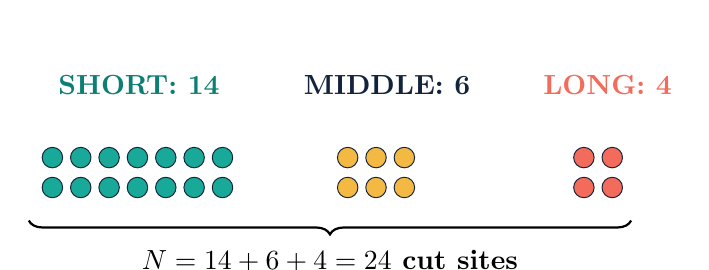
\begin{tikzpicture}[every node/.style={font=\small,align=center}]
  \node[font=\bfseries,text=tealdark] at (1.1,1.3) {SHORT: 14};
  \foreach \x in {0,...,6}{
    \foreach \y in {0,1}{
      \filldraw[fill=teal,draw=navy,line width=0.35pt] (\x*0.36,\y*0.38) circle (0.13);
    }
  }
  \node[font=\bfseries,text=navy] at (4.25,1.3) {MIDDLE: 6};
  \foreach \x in {0,...,2}{
    \foreach \y in {0,1}{
      \filldraw[fill=gold,draw=navy,line width=0.35pt] (3.75+\x*0.36,\y*0.38) circle (0.13);
    }
  }
  \node[font=\bfseries,text=coral] at (7.05,1.3) {LONG: 4};
  \foreach \x in {0,...,1}{
    \foreach \y in {0,1}{
      \filldraw[fill=coral,draw=navy,line width=0.35pt] (6.75+\x*0.36,\y*0.38) circle (0.13);
    }
  }
  \draw[decorate,decoration={brace,amplitude=5pt,mirror},thick] (-0.3,-0.42) -- (7.35,-0.42)
    node[midway,below=7pt,font=\bfseries] {\(N=14+6+4=24\) cut sites};
\end{tikzpicture}
\caption{The multinomial asks how one fixed total is allocated across categories. These are the same 24 observations, not 24 new observations.}
\end{figure}

If the expected bin probabilities are
\[
\boldsymbol{\rho}=(0.50,\ 0.30,\ 0.20),
\]
then the expected counts for \(N=30\) are
\[
30\boldsymbol{\rho}=(15,\ 9,\ 6).
\]
The observed split can differ because it is random.

\begin{checkpoint}
Which model answers each question?

\begin{enumerate}[leftmargin=2em]
  \item Why was the total count 24 instead of 20 or 30?
  \item Given that the total was 24, why did it split 14/6/4?
\end{enumerate}

Answer: the negative binomial addresses question 1; the conditional multinomial
addresses question 2.
\end{checkpoint}

\subsection{Gamma: a distribution on positive values}

An effective abundance cannot be negative. A Gamma distribution lives only on
positive numbers, so it is a natural prior for abundance.

\begin{figure}[H]
\centering
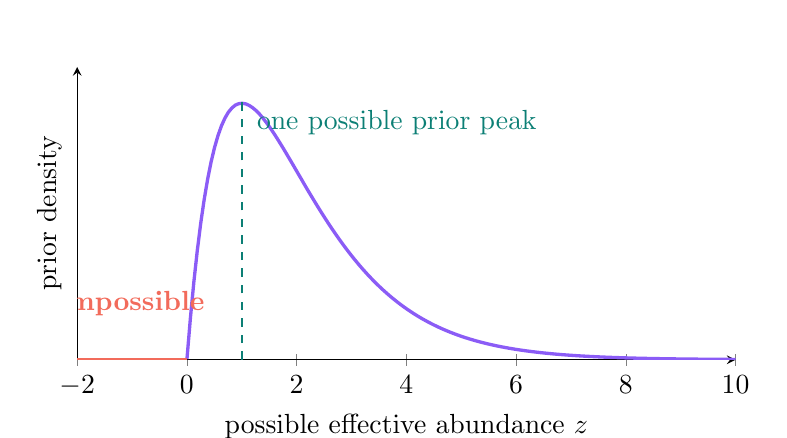
\begin{tikzpicture}
\begin{axis}[
  width=0.82\linewidth,
  height=5.3cm,
  xmin=-2,xmax=10,
  ymin=0,ymax=0.42,
  xlabel={possible effective abundance \(z\)},
  ylabel={prior density},
  ytick=\empty,
  axis lines=left,
  samples=160
]
\addplot[domain=0.001:10,very thick,purple] {x*exp(-x)};
\addplot[domain=-2:0,very thick,coral] {0};
\draw[dashed,tealdark,thick] (axis cs:1,0) -- (axis cs:1,0.38);
\node[anchor=west,text=tealdark] at (axis cs:1.1,0.34) {one possible prior peak};
\node[text=coral,font=\bfseries] at (axis cs:-1,0.08) {impossible};
\end{axis}
\end{tikzpicture}
\caption{A Gamma density is zero at negative values. The exact curve depends on its hyperparameters; this one is only an illustration.}
\end{figure}

\begin{bigidea}
The three distributions have three different jobs:
\[
\boxed{
\begin{array}{rcl}
\text{negative binomial} &:& \text{How many cuts?}\\
\text{multinomial} &:& \text{How are those cuts divided?}\\
\text{Gamma} &:& \text{Which positive abundances were plausible beforehand?}
\end{array}}
\]
\end{bigidea}

\section{A mixture is a weighted recipe}

\subsection{Reference fingerprints}

Start with two simplified reference types at one peak:

\begin{center}
\begin{tabular}{L{0.30\linewidth}C{0.20\linewidth}C{0.20\linewidth}C{0.18\linewidth}}
\toprule
Reference & Short & Long & Total \\
\midrule
T cell & 80\% & 20\% & 100 \\
B cell & 20\% & 80\% & 100 \\
\bottomrule
\end{tabular}
\end{center}

Both types have the same total accessibility in this teaching example. A
count-only model sees no difference. Their length patterns, however, are very
different.

\subsection{Solve a tiny mixture}

Suppose an observed spot is 60\% short and 40\% long. Let \(\pi_T\) be the T-cell
proportion. Then the B-cell proportion is \(1-\pi_T\). The expected short fraction
is a weighted average:
\[
0.60=0.80\pi_T+0.20(1-\pi_T).
\]
Solve:
\[
\begin{aligned}
0.60&=0.80\pi_T+0.20-0.20\pi_T,\\
0.40&=0.60\pi_T,\\
\pi_T&=\frac{2}{3}\approx0.67.
\end{aligned}
\]
So the spot looks like roughly 67\% T and 33\% B.

\begin{figure}[H]
\centering
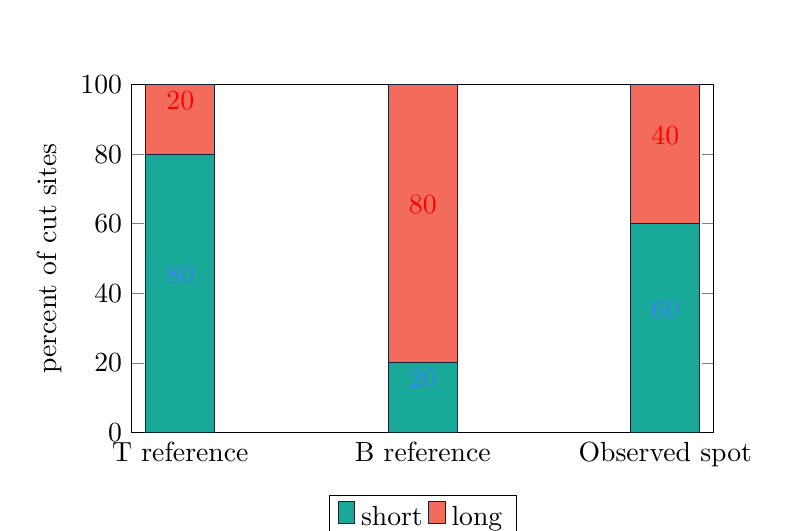
\begin{tikzpicture}
\begin{axis}[
  ybar stacked,
  bar width=25pt,
  width=0.74\linewidth,
  height=6.0cm,
  ymin=0,ymax=100,
  ylabel={percent of cut sites},
  symbolic x coords={T reference,B reference,Observed spot},
  xtick=data,
  legend style={at={(0.5,-0.18)},anchor=north,legend columns=2},
  nodes near coords,
  nodes near coords align={vertical}
]
\addplot+[fill=teal,draw=navy] coordinates {(T reference,80) (B reference,20) (Observed spot,60)};
\addplot+[fill=coral,draw=navy] coordinates {(T reference,20) (B reference,80) (Observed spot,40)};
\legend{short,long}
\end{axis}
\end{tikzpicture}
\caption{The observed length pattern lies between the two reference patterns. A weighted recipe explains where.}
\end{figure}

\begin{watchout}
This exact algebra treats observed fractions like expected fractions so the idea is
easy to see. A probability model is still needed because real observed counts
wiggle around their expectations.
\end{watchout}

\begin{checkpoint}
If a spot is 75\% T and 25\% B, what short fraction is expected?
\[
0.75(0.80)+0.25(0.20)=0.65.
\]
The answer is 65\%.
\end{checkpoint}

\section{The generative story: run the model forward}

\term{Generative} means the model describes how data could be generated. It does
not claim that scientists literally watch nature execute these steps. The steps
organize assumptions so they can be checked.

\begin{figure}[H]
\centering
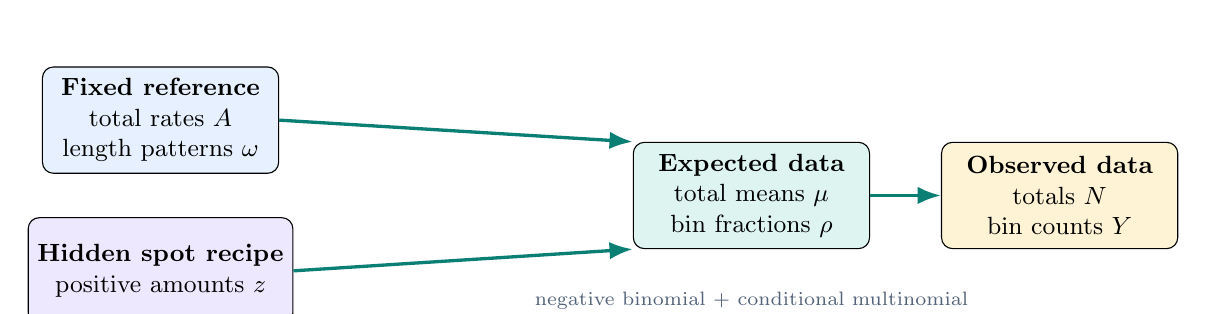
\begin{tikzpicture}[>=Latex,node distance=1.0cm,every node/.style={font=\small,align=center}]
  \node[draw,rounded corners,fill=bluepale,minimum width=3.0cm,minimum height=1.35cm] (ref) {
    \textbf{Fixed reference}\\
    total rates \(A\)\\
    length patterns \(\omega\)
  };
  \node[draw,rounded corners,fill=purplepale,minimum width=3.0cm,minimum height=1.35cm,below=0.55cm of ref] (z) {
    \textbf{Hidden spot recipe}\\
    positive amounts \(z\)
  };
  \coordinate (inputmid) at ($(ref.east)!0.5!(z.east)$);
  \node[draw,rounded corners,fill=tealpale,minimum width=3.0cm,minimum height=1.35cm,right=4.4cm of inputmid] (exp) {
    \textbf{Expected data}\\
    total means \(\mu\)\\
    bin fractions \(\rho\)
  };
  \node[draw,rounded corners,fill=goldpale,minimum width=3.0cm,minimum height=1.35cm,right=0.9cm of exp] (obs) {
    \textbf{Observed data}\\
    totals \(N\)\\
    bin counts \(Y\)
  };
  \draw[->,very thick,tealdark] (ref.east) -- (exp.north west);
  \draw[->,very thick,tealdark] (z.east) -- (exp.south west);
  \draw[->,very thick,tealdark] (exp) -- (obs);
  \node[below=0.42cm of exp,font=\scriptsize,text=slate] {negative binomial + conditional multinomial};
\end{tikzpicture}
\caption{The forward direction. Inference observes the right side and searches for a supported value of \(z\).}
\end{figure}

One pass through the story is:

\begin{enumerate}[leftmargin=2em]
  \item Choose possible positive cell-type amounts \(z\) according to a prior.
  \item Combine \(z\) with the fixed reference total rates \(A\) to calculate an expected peak total \(\mu\).
  \item Combine \(z\), \(A\), and reference length patterns \(\omega\) to calculate expected bin fractions \(\rho\).
  \item Draw a noisy total \(N\) from a negative binomial.
  \item Given \(N\), draw the bin counts \(Y\) from a multinomial.
\end{enumerate}

\begin{translation}
Forward question: “If this proposed mixture were true, what data could it
produce?”

Inference question: “Among all proposed mixtures, which ones make the observed
data plausible and also agree reasonably with the prior?”
\end{translation}

\subsection{Candidate explanations receive scores}

The computer tries candidate abundance values, calculates their expected data,
and scores them:

\begin{figure}[H]
\centering
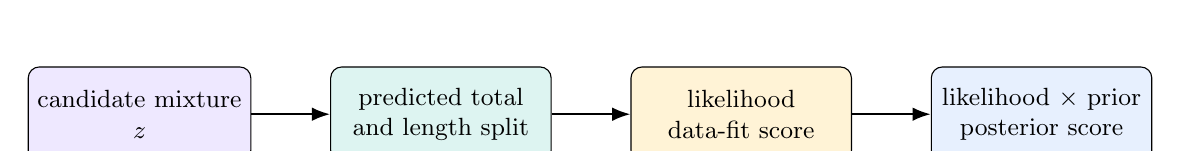
\begin{tikzpicture}[>=Latex,every node/.style={font=\small,align=center}]
  \node[draw,rounded corners,fill=purplepale,minimum width=2.8cm,minimum height=1.2cm] (candidate) {candidate mixture\\\(z\)};
  \node[draw,rounded corners,fill=tealpale,minimum width=2.8cm,minimum height=1.2cm,right=1.0cm of candidate] (predict) {predicted total\\and length split};
  \node[draw,rounded corners,fill=goldpale,minimum width=2.8cm,minimum height=1.2cm,right=1.0cm of predict] (like) {likelihood\\data-fit score};
  \node[draw,rounded corners,fill=bluepale,minimum width=2.8cm,minimum height=1.2cm,right=1.0cm of like] (post) {likelihood \(\times\) prior\\posterior score};
  \draw[->,thick] (candidate) -- (predict);
  \draw[->,thick] (predict) -- (like);
  \draw[->,thick] (like) -- (post);
\end{tikzpicture}
\caption{Bayesian computation compares explanations by combining data fit with prior plausibility.}
\end{figure}

\section{Learn to read the notation}

Mathematical notation is compressed language. Decode one piece at a time instead
of trying to understand an entire equation in one glance.

\subsection{Indices are addresses}

\begin{center}
\begin{tabular}{C{0.12\linewidth}L{0.66\linewidth}}
\toprule
Index & Address component \\
\midrule
\(s\) & spatial spot or pseudo-spot \\
\(p\) & genomic peak \\
\(b\) & parent-fragment length bin: short, middle, or long \\
\(c\) & reference cell type \\
\bottomrule
\end{tabular}
\end{center}

Thus \(Y_{3,12,2}\) means:

\begin{quote}
the observed cut-site count in spot 3, peak 12, length bin 2.
\end{quote}

\subsection{Sums, vectors, and dots}

\[
N_{s,p}=\sum_bY_{s,p,b}
\]
means: hold spot \(s\) and peak \(p\) fixed, then add the counts over all bins
\(b\).

If
\[
\boldsymbol{Y}_{s,p,\boldsymbol{\cdot}}=(14,6,4),
\]
the bold symbol represents the whole three-number vector. The dot means “all
values along this index.” Its total is \(N_{s,p}=24\).

\subsection{A small notation dictionary}

\begin{center}
\begin{tabularx}{0.96\linewidth}{C{0.13\linewidth}L{0.25\linewidth}X}
\toprule
Symbol & Read it as & Meaning \\
\midrule
\(\sum_c\) & sum over cell types & Add one contribution from every cell type. \\
\(A\mid B\) & A given B & Treat B as already known or fixed. \\
\(\propto\) & proportional to & Equal up to a shared normalizing constant. \\
\(\sim\) & follows a distribution & A random draw is modeled by the named distribution. \\
\(\E[X]\) & expected value of X & The long-run average or model mean. \\
\(\Var(X)\) & variance of X & A measure of spread around the mean. \\
\(\log x\) & log of x & Turns products into sums and helps numerical stability. \\
\(\arg\max_z f(z)\) & z that maximizes f & The input value at the highest point of the function. \\
\(\widehat z\) & z-hat & An estimated value of \(z\). \\
\bottomrule
\end{tabularx}
\end{center}

\subsection{Data, parameters, inputs, and calculated quantities}

\begin{longtable}{L{0.13\linewidth}L{0.41\linewidth}L{0.33\linewidth}}
\caption{The primary ShapeMix quantities in beginner language.}\label{tab:symbols}\\
\toprule
Symbol & Meaning & Role \\
\midrule
\endfirsthead
\toprule
Symbol & Meaning & Role \\
\midrule
\endhead
\(Y_{s,p,b}\) & cut sites observed in one length bin & observed data \\
\(N_{s,p}\) & all cut sites observed in the peak, \(\sum_bY_{s,p,b}\) & observed, calculated from \(Y\) \\
\(A_{c,p}\) & typical total cut-site rate for reference type \(c\) at peak \(p\) & fixed reference input \\
\(\omega_{c,p,b}\) & typical fraction in bin \(b\) for that type and peak & fixed reference input \\
\(\phi_{\mathrm{ref}}\) & reference inverse-dispersion controlling extra total-count noise & fixed reference input \\
\(z_{s,c}\) & positive, effective amount of cell type \(c\) in spot \(s\) & unknown parameter inferred by MAP \\
\(e_s\) & total effective abundance, \(\sum_cz_{s,c}\) & calculated \\
\(\mu_{s,p}\) & expected total cut-site count & calculated \\
\(\rho_{s,p,b}\) & expected fraction of cuts in bin \(b\) & calculated \\
\(\pi_{s,c}\) & normalized cell-type proportion, \(z_{s,c}/e_s\) & reported output \\
\bottomrule
\end{longtable}

\begin{watchout}
\(z_{s,c}\) is not a calibrated nucleus count: it need not be an integer or sum
to the number of cells used to simulate a pseudo-spot. In this model it is an
effective, depth-scaled reference-cell-equivalent abundance. The primary
biological output is the normalized proportion \(\pi_{s,c}\).
\end{watchout}

\subsection{Parameter versus hyperparameter}

A \term{parameter} is an unknown value the model infers, such as \(z_{s,c}\). A
\term{hyperparameter} is a fixed setting that controls a prior or another piece of
model behavior, such as \(r_z\), \(m_c\), or a smoothing strength.

\begin{checkpoint}
Is \(\mu_{s,p}\) an independently inferred parameter? No. Once \(z\) and the fixed
reference \(A\) are known, \(\mu\) is calculated deterministically.
\end{checkpoint}

\section{A complete ShapeMix example with small numbers}

\subsection{Set up the reference}

Use one peak, two cell types, and three length bins. Let both reference types have
the same total rate:
\[
A_T=A_B=6\text{ cuts per effective reference unit}.
\]
Their conditional length fingerprints differ:
\[
\boldsymbol{\omega}_T=
\left(\frac12,\frac13,\frac16\right),
\qquad
\boldsymbol{\omega}_B=
\left(\frac16,\frac13,\frac12\right).
\]

In words, T-cell cuts tend to have short parents, B-cell cuts tend to have long
parents, and both have one-third middle-parent cuts.

\subsection{Try one hidden mixture}

Suppose the candidate abundance is
\[
z_T=3,\qquad z_B=1.
\]
Its normalized proportions are
\[
\pi_T=\frac{3}{3+1}=0.75,\qquad
\pi_B=\frac{1}{3+1}=0.25.
\]

First compute the expected total:
\[
\mu=z_TA_T+z_BA_B=3(6)+1(6)=24.
\]

Now compute each expected bin count \(v_b\):
\[
\begin{aligned}
v_{\text{short}}
&=3(6)\left(\frac12\right)+1(6)\left(\frac16\right)
=9+1=10,\\
v_{\text{middle}}
&=3(6)\left(\frac13\right)+1(6)\left(\frac13\right)
=6+2=8,\\
v_{\text{long}}
&=3(6)\left(\frac16\right)+1(6)\left(\frac12\right)
=3+3=6.
\end{aligned}
\]
Check conservation:
\[
10+8+6=24=\mu.
\]

Finally divide by the total to obtain multinomial probabilities:
\[
\boldsymbol{\rho}
=\frac{(10,8,6)}{24}
=\left(\frac{5}{12},\frac13,\frac14\right).
\]

\begin{figure}[H]
\centering
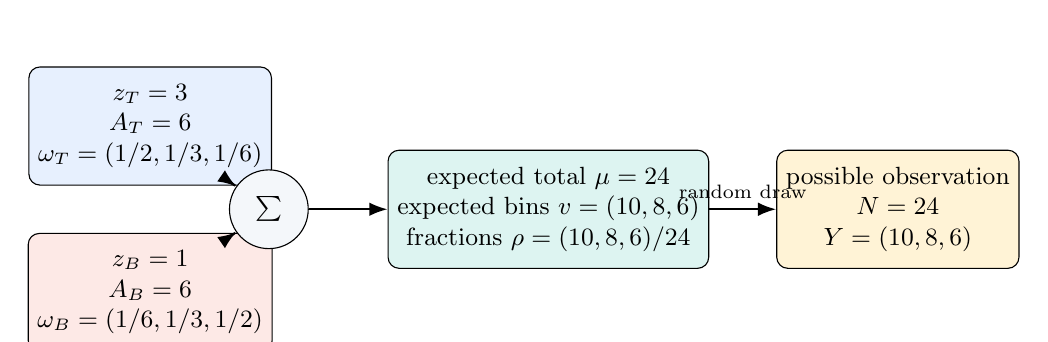
\begin{tikzpicture}[>=Latex,every node/.style={font=\small,align=center}]
  \node[draw,rounded corners,fill=bluepale,minimum width=3.0cm,minimum height=1.5cm] (t) {
    \(z_T=3\)\\
    \(A_T=6\)\\
    \(\omega_T=(1/2,1/3,1/6)\)
  };
  \node[draw,rounded corners,fill=coralpale,minimum width=3.0cm,minimum height=1.5cm,below=0.6cm of t] (b) {
    \(z_B=1\)\\
    \(A_B=6\)\\
    \(\omega_B=(1/6,1/3,1/2)\)
  };
  \node[draw,circle,fill=pale,minimum size=1.0cm,right=1.0cm of $(t)!0.5!(b)$] (sum) {\(\sum\)};
  \node[draw,rounded corners,fill=tealpale,minimum width=3.1cm,minimum height=1.5cm,right=1.0cm of sum] (expected) {
    expected total \(\mu=24\)\\
    expected bins \(v=(10,8,6)\)\\
    fractions \(\rho=(10,8,6)/24\)
  };
  \node[draw,rounded corners,fill=goldpale,minimum width=2.6cm,minimum height=1.5cm,right=0.85cm of expected] (obs) {
    possible observation\\
    \(N=24\)\\
    \(Y=(10,8,6)\)
  };
  \draw[->,thick] (t) -- (sum);
  \draw[->,thick] (b) -- (sum);
  \draw[->,thick] (sum) -- (expected);
  \draw[->,thick] (expected) -- node[above,font=\scriptsize]{random draw} (obs);
\end{tikzpicture}
\caption{A complete one-peak calculation. The observation happens to equal the expectation here so the arithmetic is easy to follow; real observations fluctuate.}
\end{figure}

\begin{bigidea}
Both models observe \(N=24\). With \(A_T=A_B\) and total effective abundance
\(e=z_T+z_B=4\) held fixed, count-only predicts \(\mu=24\) for every T/B split.
ShapeMix also predicts the split \((10,8,6)\), which depends on the mixture
because \(\omega_T\neq\omega_B\).
\end{bigidea}

\subsection{Connect back to fragments}

If all fragment ends are assigned to this same peak, the observed
\[
Y=(10,8,6)
\]
can be pictured as 5 short, 4 middle, and 3 long fragments. That is 12 fragments
and \(2\times12=24\) cut-site counts.

\section{The two-part ShapeMix likelihood}

\subsection{One joint story, factored into two questions}

ShapeMix writes the data model as
\[
\boxed{
p(N,Y\mid z,A,\omega,\phi_{\mathrm{ref}})
=
p(N\mid z,A,\phi_{\mathrm{ref}})
\;p(Y\mid N,z,A,\omega).
}
\]

This is the probability product rule: model the total, then model the split
conditional on that total.

\begin{figure}[H]
\centering
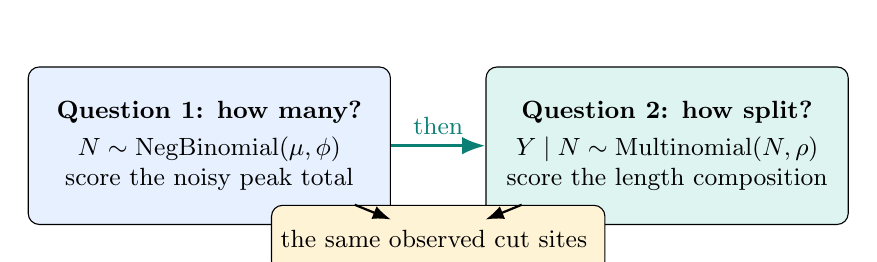
\begin{tikzpicture}[>=Latex,every node/.style={font=\small,align=center}]
  \node[draw,rounded corners,fill=bluepale,minimum width=4.6cm,minimum height=2.0cm] (nb) {
    \textbf{Question 1: how many?}\\[0.25em]
    \(N\sim\NB(\mu,\phi)\)\\
    score the noisy peak total
  };
  \node[draw,rounded corners,fill=tealpale,minimum width=4.6cm,minimum height=2.0cm,right=1.2cm of nb] (multi) {
    \textbf{Question 2: how split?}\\[0.25em]
    \(Y\mid N\sim\Mult(N,\rho)\)\\
    score the length composition
  };
  \draw[->,very thick,tealdark] (nb) -- node[above]{then} (multi);
  \node[draw,rounded corners,fill=goldpale,minimum width=4.0cm,minimum height=0.85cm,below=0.75cm of $(nb)!0.5!(multi)$] (same) {
    the same observed cut sites
  };
  \draw[->,thick] (same) -- (nb);
  \draw[->,thick] (same) -- (multi);
\end{tikzpicture}
\caption{The likelihood separates total-count information from conditional shape information without inventing extra observations.}
\end{figure}

\begin{watchout}
Using \(N\) and \(Y\mid N\) does not double-count the data. It is a factorization
of one joint probability. The negative binomial asks why the sum had its observed
value; the conditional multinomial asks how that fixed sum was allocated.
\end{watchout}

\subsection{The two model arms}

The count-only objective uses
\[
\log p(N\mid z,A,\phi_{\mathrm{ref}})+\log p(z).
\]
ShapeMix uses
\[
\log p(N\mid z,A,\phi_{\mathrm{ref}})
+\log p(Y\mid N,z,A,\omega)
+\log p(z).
\]
Everything except the conditional shape term is kept the same.

\begin{center}
\begin{tabular}{L{0.27\linewidth}C{0.16\linewidth}C{0.16\linewidth}L{0.27\linewidth}}
\toprule
Ingredient & Count-only & ShapeMix & Purpose \\
\midrule
Negative-binomial total & yes & yes & same peak-count evidence \\
Conditional multinomial & no & yes & extra length-bin evidence \\
Gamma prior on \(z\) & yes & yes & same regularization \\
Data, references, optimizer & same & same & fair comparison \\
\bottomrule
\end{tabular}
\end{center}

\begin{checkpoint}
If every cell type has exactly the same \(\omega\), can shape help identify the
mixture? No. Then \(\rho\) does not change with \(z\), so the conditional shape
term contains no mixture information.
\end{checkpoint}

\section{The prior: make assumptions visible}

\subsection{Why use a prior?}

Observed data may be noisy or ambiguous. A prior gives the model a transparent
starting preference before the current spot is examined. For ShapeMix, it also
enforces an essential fact: abundance must be positive.

The primary model uses
\[
\boxed{
z_{s,c}\sim
\Gam\left(
\text{shape}=r_z,\;
\text{rate}=\frac{r_z}{m_c}
\right).
}
\]
Under this \term{shape--rate} convention,
\[
\E[z_{s,c}]=m_c,
\qquad
\Var(z_{s,c})=\frac{m_c^2}{r_z}.
\]

The general symbols make the prior's roles visible. Under the frozen MVP v1
evaluation contract, \(r_z=2\) and \(m_c=2\) for every cell type, so
\[
z_{s,c}\sim\Gam(\text{shape}=2,\text{rate}=1).
\]

\begin{translation}
\(m_c\) sets the prior mean for the effective abundance of cell type \(c\).
Larger \(r_z\) makes the prior more concentrated around that mean; smaller \(r_z\)
makes it broader. Both are fixed before final evaluation.
\end{translation}

\begin{watchout}
Some books define a Gamma distribution using a \emph{scale} instead of a
\emph{rate}. The target ShapeMix tutorial uses shape and rate. The second argument
\(r_z/m_c\) is a rate.
\end{watchout}

\subsection{The prior is neither cheating nor certainty}

\begin{figure}[H]
\centering
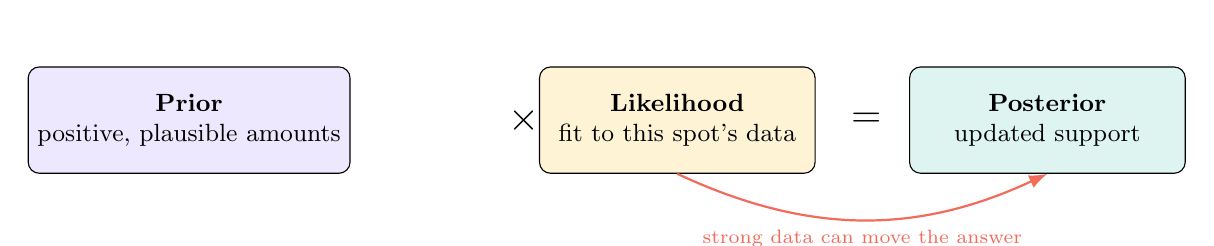
\begin{tikzpicture}[>=Latex,every node/.style={font=\small,align=center}]
  \node[draw,rounded corners,fill=purplepale,minimum width=3.5cm,minimum height=1.35cm] (prior) {
    \textbf{Prior}\\
    positive, plausible amounts
  };
  \node[font=\Large] at (4.25,0) {\(\times\)};
  \node[draw,rounded corners,fill=goldpale,minimum width=3.5cm,minimum height=1.35cm] (like) at (6.2,0) {
    \textbf{Likelihood}\\
    fit to this spot's data
  };
  \node[font=\Large] at (8.6,0) {\(=\)};
  \node[draw,rounded corners,fill=tealpale,minimum width=3.5cm,minimum height=1.35cm] (post) at (10.9,0) {
    \textbf{Posterior}\\
    updated support
  };
  \draw[->,thick,coral,bend right=25] (like.south) to node[below,font=\scriptsize]{strong data can move the answer} (post.south);
\end{tikzpicture}
\caption{The posterior balances prior plausibility with data fit. Neither component should be hidden.}
\end{figure}

With little data, many mixtures can fit and the prior has more influence. With
strong, consistent data, the likelihood becomes sharply different across
candidates and can pull the posterior away from the prior.

\begin{checkpoint}
Which is a parameter: \(z_{s,c}\) or \(r_z\)? \(z_{s,c}\) is inferred, so it is a
parameter. \(r_z\) controls its prior and is fixed, so it is a hyperparameter.
\end{checkpoint}

\section{Posterior and MAP: find the highest-supported mixture}

\subsection{A teaching grid of candidate mixtures}

Return to the three-bin example:
\[
\omega_T=(1/2,1/3,1/6),\qquad
\omega_B=(1/6,1/3,1/2),\qquad
Y=(10,8,6).
\]

To make the update visible, temporarily consider only five possible T-cell
proportions and give them equal prior probability. The conditional multinomial
likelihood supplies the data-fit score.

\begin{center}
\begin{tabular}{C{0.16\linewidth}C{0.28\linewidth}C{0.22\linewidth}}
\toprule
Candidate \(\pi_T\) & Expected short/middle/long at \(N=24\) & Posterior support on grid \\
\midrule
0\% & \(4/8/12\) & 0.3\% \\
25\% & \(6/8/10\) & 5.7\% \\
50\% & \(8/8/8\) & 26.4\% \\
75\% & \(10/8/6\) & \textbf{43.8\%} \\
100\% & \(12/8/4\) & 23.8\% \\
\bottomrule
\end{tabular}
\end{center}

\begin{figure}[H]
\centering
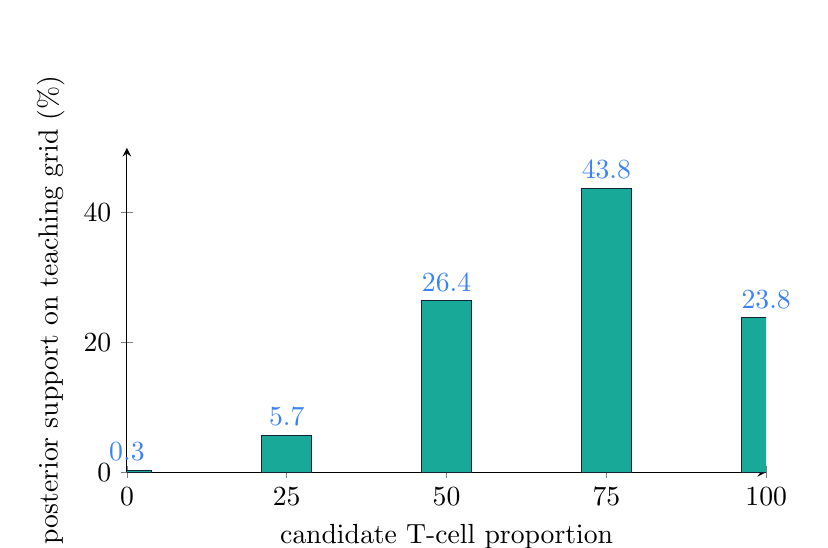
\begin{tikzpicture}
\begin{axis}[
  ybar,
  bar width=18pt,
  width=0.80\linewidth,
  height=5.7cm,
  ymin=0,ymax=50,
  ylabel={posterior support on teaching grid (\%)},
  xlabel={candidate T-cell proportion},
  symbolic x coords={0,25,50,75,100},
  xtick=data,
  nodes near coords,
  nodes near coords align={vertical},
  axis lines=left
]
\addplot+[fill=teal,draw=navy] coordinates {(0,0.3) (25,5.7) (50,26.4) (75,43.8) (100,23.8)};
\end{axis}
\end{tikzpicture}
\caption{The 75\% T candidate has the largest posterior support among these five choices, so it is the grid MAP. Other candidates retain nonzero support.}
\end{figure}

\begin{watchout}
This five-point grid is only for teaching. The real model searches continuous
positive abundance values \(z\) and uses the Gamma prior, not five equally likely
percentages.
\end{watchout}

\subsection{What MAP means}

MAP stands for \term{maximum a posteriori}. It is the parameter value at the
highest point of the posterior density:
\[
\boxed{
\widehat z_{\mathrm{MAP}}
=
\arg\max_{z>0}p(z\mid N,Y,A,\omega,\phi_{\mathrm{ref}}).
}
\]

Because the logarithm is an increasing function, the same maximum is found by
maximizing the log posterior:
\[
\widehat z_{\mathrm{MAP}}
=
\arg\max_{z>0}
\left[
\log p(N\mid z)
+\log p(Y\mid N,z)
+\log p(z)
\right].
\]

\begin{bigidea}
Logs are useful because:

\begin{enumerate}[leftmargin=2em]
  \item multiplication becomes addition, and
  \item extremely small probability products are easier for a computer to handle.
\end{enumerate}
\end{bigidea}

\subsection{The hill-climbing picture}

\begin{figure}[H]
\centering
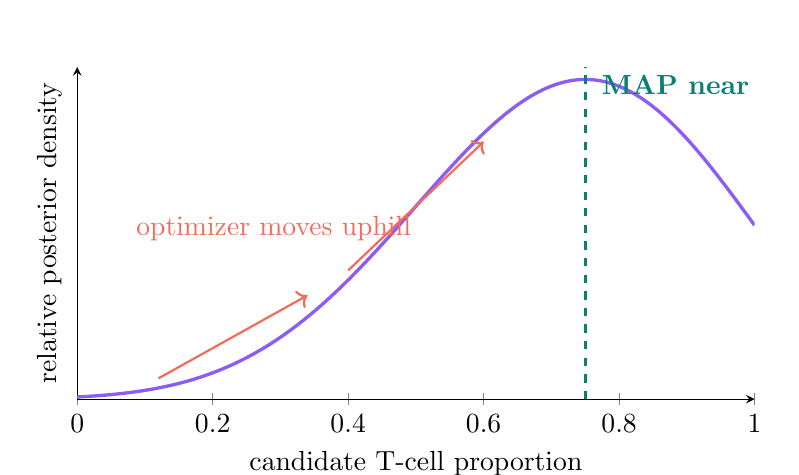
\begin{tikzpicture}
\begin{axis}[
  width=0.84\linewidth,
  height=5.8cm,
  xmin=0,xmax=1,
  ymin=0,
  xlabel={candidate T-cell proportion},
  ylabel={relative posterior density},
  ytick=\empty,
  axis lines=left,
  samples=160
]
\addplot[domain=0:1,very thick,purple] {100000000*(1/6+x/3)^10*(1/2-x/3)^6};
\addplot[dashed,tealdark,very thick] coordinates {(0.75,0) (0.75,4.0)};
\node[anchor=south west,text=tealdark,font=\bfseries] at (axis cs:0.76,3.55) {MAP near 0.75};
\draw[->,thick,coral] (axis cs:0.12,0.25) -- (axis cs:0.34,1.25);
\draw[->,thick,coral] (axis cs:0.40,1.55) -- (axis cs:0.60,3.10);
\node[text=coral] at (axis cs:0.29,2.05) {optimizer moves uphill};
\end{axis}
\end{tikzpicture}
\caption{A schematic continuous posterior for the same multinomial example with a flat prior. The optimizer searches for the highest point.}
\end{figure}

\subsection{What MAP does not provide}

The primary ShapeMix MVP reports one MAP point estimate. It does \emph{not} report:

\begin{itemize}[leftmargin=2em]
  \item a posterior mean,
  \item samples from the full posterior,
  \item a credible interval, or
  \item calibrated uncertainty for each cell type.
\end{itemize}

\begin{watchout}
Calling a method Bayesian describes how the prior and likelihood define a
posterior. Using MAP summarizes that posterior by one point. Do not turn a MAP
point into an uncertainty claim it does not support.
\end{watchout}

\section{The full primary model, translated line by line}

\subsection{First calculate expected contributions}

\[
\boxed{
v_{s,p,b}=\sum_cz_{s,c}A_{c,p}\omega_{c,p,b}
}
\]

\begin{translation}
For one spot, peak, and length bin: multiply each cell type's effective amount by
its typical total rate and its typical fraction in this bin; then add across cell
types.
\end{translation}

\[
\boxed{
\mu_{s,p}=\sum_bv_{s,p,b}=\sum_cz_{s,c}A_{c,p}
}
\]

\begin{translation}
Add the expected bin contributions to get the expected total cut-site count.
Because each \(\omega_{c,p,\boldsymbol{\cdot}}\) sums to one, the length fractions
disappear from the total.
\end{translation}

\[
\boxed{
\rho_{s,p,b}=\frac{v_{s,p,b}}{\mu_{s,p}}
}
\]

\begin{translation}
Divide one expected bin count by the expected total. The resulting
\(\rho_{s,p,\boldsymbol{\cdot}}\) values are nonnegative and sum to one.
\end{translation}

\subsection{Then model the observations}

\[
\boxed{
N_{s,p}
\sim
\NB\left(
\text{mean}=\mu_{s,p},\
\text{inverse-dispersion}
=\max(e_s,\epsilon)\phi_{\mathrm{ref}}
\right)
}
\]

\begin{translation}
The peak total is a noisy count around \(\mu_{s,p}\). Here
\(e_s=\sum_cz_{s,c}\). The small fixed \(\epsilon>0\) is a numerical safety floor.
\end{translation}

\[
\boxed{
\boldsymbol{Y}_{s,p,\boldsymbol{\cdot}}\mid N_{s,p}
\sim
\Mult\left(
N_{s,p},\boldsymbol{\rho}_{s,p,\boldsymbol{\cdot}}
\right)
}
\]

\begin{translation}
Once the observed total is fixed, split those same cut sites among the three
parent-length bins according to the predicted fractions \(\rho\).
\end{translation}

\subsection{Add the prior and report proportions}

\[
z_{s,c}\sim\Gam\left(r_z,\frac{r_z}{m_c}\right),
\qquad
\pi_{s,c}=\frac{z_{s,c}}{\sum_{c'}z_{s,c'}}.
\]

\begin{translation}
The Gamma prior keeps abundance positive and regularized. Normalize the inferred
effective abundances so the reported cell-type proportions sum to one. In the
frozen MVP v1, the prior is \(\Gam(2,1)\) for every cell type.
\end{translation}

\subsection{Bayes' rule for this exact model}

\[
\boxed{
p(z\mid N,Y,A,\omega,\phi_{\mathrm{ref}})
\propto
\underbrace{p(N\mid z,A,\phi_{\mathrm{ref}})}_{\substack{\text{total-count}\\\text{likelihood}}}
\;\times\;
\underbrace{p(Y\mid N,z,A,\omega)}_{\substack{\text{conditional shape}\\\text{likelihood}}}
\;\times\;
\underbrace{p(z)}_{\substack{\text{Gamma}\\\text{prior}}}.
}
\]

\begin{bigidea}
The only inferred biological parameter in the primary model is \(z\).
\(A\), \(\omega\), and \(\phi_{\mathrm{ref}}\) are estimated from training
reference cells and then held fixed. \(\mu\), \(\rho\), \(e\), and \(\pi\) are
calculated from those quantities.
\end{bigidea}

\section{How to read the advanced ShapeMix tutorial}

The destination document is:

\begin{center}
\texttt{ShapeMix\_ATAC\_Bayesian\_Model\_Tutorial.pdf}
\end{center}

Its equations are compact because it assumes most of this companion material.
Use three passes instead of trying to master every line at once.

\subsection{Pass 1: understand the story}

\begin{enumerate}[leftmargin=2em]
  \item Read \emph{What problem is ShapeMix-ATAC solving?}
  \item Read \emph{The data table: from peak counts to shape counts}.
  \item Read \emph{A short Bayesian warm-up}.
  \item Jump to \emph{Worked example: why shape helps}.
  \item Finish with \emph{Summary in one page}.
\end{enumerate}

In the current 18-page PDF, these are mainly viewer pages 4--5, 11--12, and
17--18. Section names are more reliable than page numbers if the PDF is rebuilt.

\subsection{Pass 2: understand the primary model}

Read these sections in order:

\begin{enumerate}[leftmargin=2em]
  \item \emph{Start with the ordinary peak-count model};
  \item \emph{The ShapeMix-ATAC likelihood};
  \item \emph{The generative story};
  \item \emph{Prior and semantics for hidden abundance};
  \item \emph{Complete core model};
  \item \emph{What the primary MAP estimate means}.
\end{enumerate}

Each time an equation appears, mark:

\begin{itemize}[leftmargin=2em]
  \item observed data in gold: \(N,Y\);
  \item fixed references in blue: \(A,\omega,\phi_{\mathrm{ref}}\);
  \item the unknown in purple: \(z\);
  \item calculated quantities in teal: \(e,\mu,\rho,\pi\).
\end{itemize}

\subsection{Pass 3: understand scientific safeguards}

Then read \emph{Reference signatures}, \emph{Leakage-free experimental structure},
\emph{Diagnostics and ablation tests}, and \emph{Fixed evaluation contract}.
These sections explain how the model is tested fairly rather than how Bayes' rule
works.

\subsection{A five-step equation-reading routine}

When an equation looks overwhelming:

\begin{enumerate}[leftmargin=2em]
  \item Identify the left side: what quantity is being defined or modeled?
  \item Label every right-side symbol as observed, fixed, inferred, or calculated.
  \item Expand one \(\sum\) using just two cell types or three bins.
  \item Ask whether the line answers “how many?”, “how split?”, or “what was plausible?”
  \item Substitute the small numbers from Section 9.
\end{enumerate}

\begin{checkpoint}
You are ready for the advanced tutorial if you can explain why
\[
p(N\mid z)\,p(Y\mid N,z)\,p(z)
\]
means “total-count fit times conditional-shape fit times prior plausibility.”
\end{checkpoint}

\newpage
\section{Practice questions}

Try these without looking at the answer key. Show the arithmetic, not only the
final answer.

\begin{enumerate}[leftmargin=2.2em,label=\textbf{\arabic*.}]
  \item Seven short, three middle, and two long fragments all have both ends in
  the same peak. What is the cut-site vector \(Y\), and what is the total \(N\)?

  \item Can a parent-length bin contain an odd number of cut-site counts in real
  data? Explain.

  \item Two hypotheses have equal priors. Their likelihoods for the observed data
  are 0.10 and 0.30. What are their normalized posterior probabilities?

  \item Explain the difference between
  \(P(\text{short}\mid T)\) and \(P(T\mid\text{short})\).

  \item If
  \[
  \boldsymbol{Y}_{s,p,\boldsymbol{\cdot}}=(6,3,1),
  \]
  what is \(N_{s,p}\)?

  \item A negative-binomial total has \(\mu=20\) and \(\phi=5\). Calculate its
  variance using the ShapeMix parameterization.

  \item Match each job to a distribution:
  \begin{enumerate}[label=(\alph*)]
    \item noisy total number of cut sites;
    \item division of a fixed total among three bins;
    \item prior for a positive effective abundance.
  \end{enumerate}

  \item In the Section 9 reference,
  \[
  \omega_T=(1/2,1/3,1/6),\quad
  \omega_B=(1/6,1/3,1/2).
  \]
  Calculate \(\rho\) for 75\% T and 25\% B.

  \item If \(z=(3,1)\), calculate the normalized proportion vector \(\pi\).

  \item Classify each quantity as observed, fixed reference, inferred, or
  calculated: \(Y\), \(A\), \(\omega\), \(z\), \(\mu\), and \(\pi\).

  \item What happens to the usefulness of the shape term if every cell type has
  the same \(\omega\)?

  \item What is the one intentional difference between the count-only and
  ShapeMix arms?

  \item Does a MAP estimate provide a credible interval? What does it provide?

  \item Give two reasons for optimizing log probabilities instead of raw
  probability products.
\end{enumerate}

\newpage
\section{Answer key}

\begin{enumerate}[leftmargin=2.2em,label=\textbf{\arabic*.}]
  \item Each fragment contributes two cut sites:
  \[
  Y=(14,6,4),\qquad N=14+6+4=24.
  \]

  \item Yes. A fragment can contribute only one selected count when one end lands
  in the peak and the other does not. Both ends inherit the same parent-length
  bin, but both are not guaranteed to be assigned to the same selected peak.

  \item The unnormalized scores are \(0.10\) and \(0.30\), totaling \(0.40\):
  \[
  0.10/0.40=0.25,\qquad0.30/0.40=0.75.
  \]

  \item \(P(\text{short}\mid T)\) predicts the chance of a short-parent cut when
  T is known. \(P(T\mid\text{short})\) infers the chance of T after short has been
  observed. Bayes' rule connects them using a prior and normalization.

  \item
  \[
  N_{s,p}=\sum_bY_{s,p,b}=6+3+1=10.
  \]

  \item
  \[
  \Var(N)=\mu+\frac{\mu^2}{\phi}
  =20+\frac{400}{5}=100.
  \]

  \item (a) negative binomial; (b) conditional multinomial; (c) Gamma.

  \item
  \[
  \begin{aligned}
  \rho
  &=0.75\omega_T+0.25\omega_B\\
  &=\left(\frac{5}{12},\frac13,\frac14\right).
  \end{aligned}
  \]
  At \(N=24\), this corresponds to expected counts \((10,8,6)\).

  \item
  \[
  \pi=\left(\frac{3}{4},\frac{1}{4}\right)=(0.75,0.25).
  \]

  \item \(Y\): observed. \(A,\omega\): fixed reference inputs. \(z\): inferred.
  \(\mu,\pi\): calculated from the inferred and fixed quantities.

  \item Shape becomes non-informative about the mixture. Changing \(z\) no longer
  changes the predicted conditional bin fractions \(\rho\).

  \item ShapeMix adds only
  \[
  \log p(Y\mid N,z,A,\omega),
  \]
  the conditional multinomial shape term. The total-count likelihood, prior,
  observations, references, initialization, optimizer, and comparison settings
  remain matched.

  \item No. MAP provides one point: the parameter setting at the highest posterior
  density found by the optimization.

  \item Logs turn products into sums, and they avoid numerical problems caused by
  multiplying many tiny probabilities.
\end{enumerate}

\newpage
\section{One-page cheat sheet}

\subsection*{Four Bayesian words}

\begin{center}
\begin{tabularx}{0.96\linewidth}{L{0.18\linewidth}X}
\toprule
Prior & Plausibility of unknown values before using the current spot's data. \\
Likelihood & How well a candidate unknown value predicts the observed data. \\
Posterior & Updated support after combining likelihood and prior. \\
MAP & The single unknown value at the highest posterior density. \\
\bottomrule
\end{tabularx}
\end{center}

\[
\boxed{\text{posterior}\propto\text{likelihood}\times\text{prior}}
\]

\subsection*{Three active distributions}

\begin{center}
\begin{tabularx}{0.96\linewidth}{L{0.26\linewidth}X}
\toprule
Negative binomial & Noisy peak total \(N\); allows more spread than Poisson. \\
Conditional multinomial & Allocation of that same fixed \(N\) among length bins. \\
Gamma & Prior on positive effective abundance \(z\). \\
\bottomrule
\end{tabularx}
\end{center}

\subsection*{Core ShapeMix flow}

\[
\boxed{
(z,A,\omega)
\longrightarrow
(\mu,\rho)
\longrightarrow
(N,Y)
}
\]

\[
v_{s,p,b}=\sum_cz_{s,c}A_{c,p}\omega_{c,p,b},
\qquad
\mu_{s,p}=\sum_bv_{s,p,b},
\qquad
\rho_{s,p,b}=\frac{v_{s,p,b}}{\mu_{s,p}}.
\]

\[
N_{s,p}\sim\NB\!\left(
\mu_{s,p},\max(e_s,\epsilon)\phi_{\mathrm{ref}}
\right),
\qquad
\boldsymbol{Y}_{s,p,\boldsymbol{\cdot}}\mid N_{s,p}
\sim\Mult(N_{s,p},\boldsymbol{\rho}_{s,p,\boldsymbol{\cdot}}).
\]

\[
z_{s,c}\sim\Gam\left(r_z,\frac{r_z}{m_c}\right),
\qquad
\pi_{s,c}=\frac{z_{s,c}}{\sum_{c'}z_{s,c'}}.
\]

For frozen MVP v1 evaluation, \(r_z=m_c=2\), so this prior is
\(\Gam(2,1)\) for every cell type.

\subsection*{Roles}

\begin{center}
\begin{tabular}{L{0.27\linewidth}L{0.58\linewidth}}
\toprule
Observed & \(Y,N\) \\
Fixed from reference & \(A,\omega,\phi_{\mathrm{ref}}\) \\
Inferred by MAP & \(z\) \\
Calculated & \(e,\mu,\rho,\pi\) \\
\bottomrule
\end{tabular}
\end{center}

\begin{bigidea}
Count-only asks how many cut sites occurred. ShapeMix asks the same question and
also asks how those same cuts were divided among parent-fragment length bins.
\end{bigidea}

\subsection*{Final readiness checklist}

You are ready to read the advanced PDF if you can:

\begin{itemize}[leftmargin=2em]
  \item distinguish \(P(E\mid H)\) from \(P(H\mid E)\);
  \item explain prior, likelihood, posterior, and MAP;
  \item identify \(Y,N,A,\omega,z,\mu,\rho,\phi,\pi\);
  \item explain the jobs of the negative binomial, multinomial, and Gamma;
  \item show why \(p(N)\,p(Y\mid N)\) is not double-counting; and
  \item explain why the MVP's MAP output is a point estimate, not a credible interval.
\end{itemize}

\section*{Relationship to the project documents}
\addcontentsline{toc}{section}{Relationship to the project documents}

This companion is an educational guide to the advanced tutorial at:
\begin{center}
\small
\texttt{docs/ShapeMix/tutorials/}\\[-0.15em]
\texttt{ShapeMix\_ATAC\_Bayesian\_Model\_Tutorial.pdf}
\end{center}
The executable model semantics are governed by
\texttt{docs/ShapeMix/model\_specification.md}. The examples here deliberately use
small numbers and simplified one-peak settings; they teach the model's logic but
are not study results.

\end{document}
